% AJ manuscript -- AASTeX. Compile with: latexmk -pdf main.tex  (needs aastex701.cls)
% Draft generated 2026-06-16. Numbers from the frozen DES test split unless noted.
\documentclass[twocolumn]{aastex701}

\shorttitle{A Neural Effective-PSF Field for DES}
\shortauthors{Regier et al.}

\usepackage{tikz}
\usepackage{amsmath,amssymb,bm}
\usetikzlibrary{positioning,arrows.meta,fit,backgrounds,calc}

% Visible, greppable placeholder for results still in progress (real-data correction).
\newcommand{\placeholder}[1]{\textbf{[\textsc{placeholder}: #1]}}

\begin{document}

\title{Learning the Effective PSF: A Neural PSF Field with Amortized
Inference for DES Single-Epoch Imaging}

\author{Jeffrey Regier}
\email{regier@umich.edu}
\affiliation{Department of Statistics, University of Michigan, Ann Arbor, MI 48109, USA}

\collaboration{1}{(The LSST Dark Energy Science Collaboration)}

\begin{abstract}
Errors in the modeled point-spread-function (PSF) are a leading source of systematic error
in weak-lensing shear measurement. Per-exposure fitters (e.g., \textsc{PSFEx}, \textsc{PIFF}) represent
the PSF as a sub-pixel surface-brightness profile that must be convolved with an assumed
pixel response to predict an image. We instead target the \emph{effective} PSF (the
pixel-convolved point-source response): the quantity sampled data identify and the exact
kernel for forward-modeling galaxies. A single neural network (multi-head
attention over an exposure's stars) predicts this effective PSF at any queried position
and oversampling in one forward pass, \emph{amortizing} the per-exposure fitting that
\textsc{PSFEx} and \textsc{PIFF} repeat on every image.
On 3{,}301 frozen test exposures of Dark Energy Survey single-epoch imaging, the model
matches or exceeds \textsc{PIFF} and \textsc{PSFEx} on every reserved-star metric---size
and ellipticity residuals, shape correlation, and per-pixel goodness of fit. In a
star-anchored galaxy injection--recovery test on real data, it recovers galaxy
\emph{ellipticity}---the weak-lensing-critical quantity---without coherent bias and on par
with \textsc{PIFF}, while recovered \emph{sizes} run a few percent small. We trace this to
the flux at which the PSF is queried: the model conditions on source flux and has learned,
from training stars carrying faint unresolved neighbours, that fainter stars are more
fractionally contaminated, so its predicted PSF narrows toward the clean PSF in the bright
limit. Querying at that clean limit removes most of the size bias, returning the PSF
concentration to truth in controlled simulations where contamination is the only
flux-dependent effect.
On real data the same query brings the predicted PSF size to within $1\%$ of bright clean
stars---from a ${\sim}13\%$ second-moment excess at the median flux---and reduces the
recovered galaxy-size bias toward the protocol floor.
Color conditioning further removes a chromatic PSF-size systematic
that the baselines retain, and the model stays accurate in star-sparse exposures where
\textsc{PIFF} degrades sharply. Controlled simulations motivate two training choices: a
\emph{blend forward-model} loss that removes a size bias from unrecognized blends, and
point-source-only attention, which fixes a spin-2 representation failure triggered by
galaxy detections in the context.
\end{abstract}

\keywords{Weak gravitational lensing (1797) --- Point spread function (1349) ---
Astronomical techniques (1684) --- Convolutional neural networks (1938) ---
Sky surveys (1464)}

\section{Introduction} \label{sec:intro}

Weak gravitational lensing infers the matter distribution from coherent ${\sim}1\%$
distortions of galaxy shapes. The measurement is limited by knowledge of the PSF: any
error in the modeled PSF size or ellipticity propagates directly into the inferred shear.
Survey pipelines model the PSF per exposure by fitting that exposure's stars with a
flexible model interpolated across the focal plane \citep[\textsc{PSFEx};][]{Bertin2011}
\citep[\textsc{PIFF};][]{Jarvis2021}. This is robust but (i)~discards information shared
across exposures and nights, (ii)~degrades when few clean stars are available, and
(iii)~is purely empirical at the star positions: it does not exploit auxiliary
information such as stellar color, which sets the chromatic PSF.

We take an amortized, learning-based approach. Rather than fit each exposure's PSF from
scratch, a single network learns, across many exposures, a \emph{data-adaptive prior}
over how the PSF looks and varies, and applies it to a new exposure in one forward pass,
mapping that exposure's stars (the \emph{context}) to a continuous PSF field queryable at
arbitrary position, color, flux, and resolution. This pools information across
the training set that no single-exposure fit can access, and in principle across the
focal plane. The inferential target is
the PSF at \emph{star-free} positions, where galaxies are measured; predicting held-out
stars is the training objective and the validation instrument. We train and evaluate on
DES single-epoch data and benchmark against \textsc{PIFF} and \textsc{PSFEx} run by us
under matched conditions.

A second difference is the \emph{target} of the model. Traditional
PSF models, including \textsc{PSFEx} (super-sampled pixels) and \textsc{PIFF} (a
surface-brightness profile on the sky), represent the PSF as a continuous function on
$\mathbb{R}^2$ at finer-than-pixel resolution, which must then be convolved with an
assumed pixel-response kernel to predict what a detector records. We instead model the
\emph{effective} PSF \citep[ePSF;][]{AndersonKing2000}: the instrumental PSF already
integrated over the pixel, i.e.\ the expected fraction of a point source's light falling
in each pixel as a function of the source's sub-pixel position. The network maps a query
position (and color, flux) directly to these expected pixel values, never representing
the continuous PSF explicitly: the sense in which our PSF is \emph{implicit}. Two grounds
motivate this target. First, identifiability: from sampled data one
cannot uniquely recover the sub-pixel surface brightness without extra assumptions,
whereas the ePSF is exactly what the pixels constrain, the reason it underpins
state-of-the-art point-source astrometry and photometry \citep{AndersonKing2000,
Lauer1999, Liaudat2023}. Second, sufficiency: the ePSF as a function of source position
is a sufficient statistic for forward-modeling \emph{any} source: a galaxy's expected
pixel data is its surface brightness convolved with the ePSF, with no separate pixel
step \citep{BernsteinJarvis2002}, so the ePSF is precisely the kernel a shear pipeline
needs. The only residual is discretizing that convolution on a finite grid, which our
ability to render at arbitrary oversampling controls directly.
\begin{figure*}
\centering
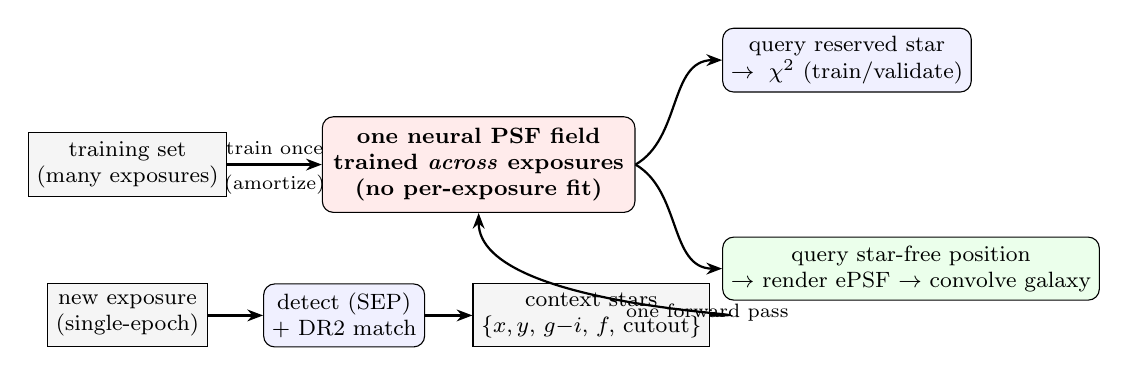
\begin{tikzpicture}[
  node distance=4mm and 8mm,
  box/.style={draw, rounded corners, align=center, minimum height=8mm,
              font=\footnotesize, fill=blue!6, inner sep=3pt},
  dat/.style={draw, align=center, minimum height=8mm, font=\footnotesize,
              fill=gray!8, inner sep=3pt},
  net/.style={draw, rounded corners, align=center, minimum height=12mm,
              font=\footnotesize\bfseries, fill=red!8, inner sep=4pt},
  outbox/.style={draw, rounded corners, align=center, minimum height=8mm,
              font=\footnotesize, fill=green!8, inner sep=3pt},
  arr/.style={-{Stealth[length=2mm]}, thick}]
% amortized training: many exposures fold into one network, once
\node[dat] (train) {training set\\(many exposures)};
\node[net, right=12mm of train] (npsf) {one neural PSF field\\trained \emph{across} exposures\\(no per-exposure fit)};
\draw[arr] (train) -- node[above, font=\scriptsize]{train once}
                     node[below, font=\scriptsize]{(amortize)} (npsf);
% deployment on a new exposure: detect -> context -> same fixed network
\node[dat, below=11mm of train] (exp) {new exposure\\(single-epoch)};
\node[box, right=7mm of exp] (det) {detect (SEP)\\+ DR2 match};
\node[dat, right=6mm of det] (ctx) {context stars\\$\{x,y,\,g{-}i,\,f,\,\mathrm{cutout}\}$};
\draw[arr] (exp)--(det); \draw[arr] (det)--(ctx);
\draw[arr] (ctx.east) to[out=0,in=-90] node[below right=-1mm and -2mm, font=\scriptsize]
  {one forward pass} (npsf.south);
% two queries of the same field
\node[box, above right=3mm and 11mm of npsf] (res)
  {query reserved star\\$\to\ \chi^2$ \footnotesize(train/validate)};
\node[outbox, below right=3mm and 11mm of npsf] (gal)
  {query star-free position\\$\to$ render ePSF $\to$ convolve galaxy};
\draw[arr] (npsf.east) to[out=30,in=180] (res.west);
\draw[arr] (npsf.east) to[out=-30,in=180] (gal.west);
\end{tikzpicture}
\caption{Overall workflow and amortization. A single network is trained once across many
exposures (top) and then applied to a new exposure in one forward pass, with no
per-exposure fitting: its detected stars (context) are mapped to a continuous PSF field
(bottom). The \emph{same} field is queried two ways: at held-out reserved stars, giving the
training objective and validation, and at star-free positions, where the rendered
(oversampled) effective PSF convolves galaxy models---the inferential target.\label{fig:workflow}}
\end{figure*}



\section{Method} \label{sec:method}
\begin{figure*}
\centering
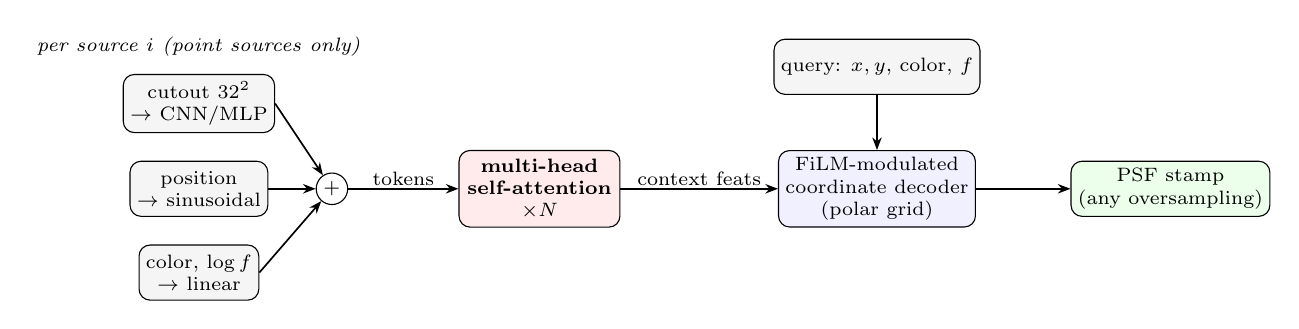
\begin{tikzpicture}[
  node distance=3.5mm and 7mm,
  enc/.style={draw, rounded corners, align=center, minimum height=7mm,
              font=\scriptsize, fill=gray!8, inner sep=2.5pt},
  op/.style={draw, circle, font=\scriptsize, inner sep=1pt, minimum size=4mm, fill=white},
  att/.style={draw, rounded corners, align=center, minimum height=9mm,
              font=\scriptsize\bfseries, fill=red!8, inner sep=3pt},
  dec/.style={draw, rounded corners, align=center, minimum height=7mm,
              font=\scriptsize, fill=blue!6, inner sep=2.5pt},
  arr/.style={-{Stealth[length=1.6mm]}, semithick}]
% per-source token encoder
\node[enc] (cut) {cutout $32^2$\\$\to$ CNN/MLP};
\node[enc, below=of cut] (pos) {position\\$\to$ sinusoidal};
\node[enc, below=of pos] (sca) {color, $\log f$\\$\to$ linear};
\node[op, right=6mm of pos] (sum) {$+$};
\draw[arr] (cut.east) -- (sum); \draw[arr] (pos.east) -- (sum); \draw[arr] (sca.east) -- (sum);
\node[align=center, font=\scriptsize, above=1mm of cut] {\emph{per source $i$ (point sources only)}};
\node[att, right=14mm of sum] (mha) {multi-head\\self-attention\\$\times N$};
\draw[arr] (sum) -- node[above, font=\scriptsize, inner sep=1pt]{tokens} (mha);
\node[dec, right=20mm of mha] (film) {FiLM-modulated\\coordinate decoder\\(polar grid)};
\draw[arr] (mha) -- node[above, font=\scriptsize, inner sep=1pt]{context feats} (film);
\node[enc, above=7mm of film] (q) {query: $x,y$, color, $f$};
\draw[arr] (q) -- (film);
\node[dec, right=12mm of film, fill=green!8] (psf) {PSF stamp\\(any oversampling)};
\draw[arr] (film) -- (psf);
\end{tikzpicture}
\caption{Network architecture. Each context source (restricted to point sources;
\S\ref{sec:method}) is encoded from its pixel cutout, sky position, and scalar
color/$\log$-flux into a token. Multi-head self-attention mixes the context; a
FiLM-modulated coordinate decoder, conditioned on the attended features and the query
(position, color, flux), renders the pixel-convolved PSF at any position and oversampling
factor.\label{fig:arch}}
\end{figure*}



\paragraph{Architecture} Each detected source is encoded from its pixel cutout (a learned
image encoder applied to the scale-normalized stamp), its sky position (sinusoidal
encoding), and scalar color and $\log$-flux. A multi-head self-attention block \citep{Vaswani2017} lets every
query attend to the context sources; a coordinate decoder then renders the PSF at the
query position and any oversampling factor, returning the pixel-convolved effective PSF
used to convolve galaxy models. The decoder uses a polar, spin-2-aware angular parametrization, with FiLM modulation
by the attended context features.

\paragraph{Inferential target (effective PSF)} The decoder outputs the effective PSF
\citep{AndersonKing2000}, the pixel-integrated point-source response, sampled at the
query grid, optionally oversampled. Because the loss below compares predicted stamps to
\emph{observed} star pixels, the model regresses the observable by construction: it
learns $\mathbb{E}[\text{pixel value}\mid\text{point source at }(x,y)]$ directly, rather
than fitting a sub-pixel profile and assuming a pixel kernel. Identifiability aligns the
three things that a non-identifiable model keeps separate: our training target, the
quantity we model, and the quantity we validate all coincide, so reserved-star residuals
(\S\ref{sec:results}) directly test what we fit. A surface-brightness model is instead
validated only through pixel- or moment-space summaries of its rendered output, the
same observable space, so its extra sub-pixel degrees of freedom are never themselves
constrained by the data. We score all three
methods on moments measured in pixel space (model stamp versus star stamp), so no method
is privileged by its internal representation. The
same pixel-convolved output is the kernel used to forward-model galaxies in
\S\ref{sec:galrec}; oversampling the render reduces the discretization error of that
convolution for compact sources.

\paragraph{Loss} Training minimizes an inverse-variance $\chi^2$ between predicted and
observed star cutouts, with the per-star amplitude solved in closed form. Star pixels are
noisy realizations whose conditional mean is the effective PSF; a squared-error objective
is minimized by the conditional expectation $\mathbb{E}[\,\text{pixel}\mid\text{source,
context}\,]$, so with enough capacity and data the objective is minimized by that
quantity, the identifiable effective PSF. The network thus targets only what the pixels
constrain, rather than a finer-than-pixel profile the sampled data do not determine. We
introduce a
\emph{blend forward-model} loss: rather than treat each clean star as isolated, we model
its cutout as a generalized-least-squares sum of the target plus its detected neighbors,
all rendered by the same decoder (\S\ref{sec:sim}). Detected galaxies near a target are
handled by exclusion (default), masking, or a crude extended-component model; the three
are within noise on real reserved stars.

\paragraph{Point-source context} The PSF should be informed only by point sources. We
restrict the attention context to stellar detections; \S\ref{sec:sim} shows this is
necessary to avoid a spin-2 corruption from extended sources in the context.

\paragraph{Color conditioning} The decoder conditions on $g{-}i$ color, enabling a
per-object chromatic PSF (differential chromatic refraction and wavelength-dependent
seeing) that per-exposure empirical models cannot represent (\S\ref{sec:chromatic}).


\section{Data} \label{sec:data}

We use DES single-epoch FITS (Y5A1, CCD~31; amplifier~B is dead, masked via MSK bit~8).
Sources are detected with \textsc{SEP} and cross-matched to DES~DR2 for colors,
\texttt{SPREAD\_MODEL} star/galaxy labels, and coadd object IDs. Splits are at the
observing-night level by deterministic hash to prevent leakage (consecutive exposures
share atmosphere), frozen in a committed manifest with ${\sim}20\%$ of clean stars per
test/validation exposure reserved for scoring only; the test split is 3{,}301 exposures
across $grizY$. Reserved stars are excluded from every method's fit/context and scored
identically across methods on the same pixel grid.

\paragraph{Simulations} A matched pipeline renders Moffat PSF fields into the same data format, with FWHM and shear
varying as second-order polynomials across the field. This variation lies within the
polynomial spatial model that \textsc{PIFF} and \textsc{PSFEx} fit, so it does not handicap
the baselines. The renderer optionally adds a chromatic dependence of FWHM on color, blended
stars, and injected galaxy detections. Star
density, galaxy density ($3{:}1$), and per-source S/N are tuned to match the real
extraction. The simulation is the controlled instrument for the systematics studies in
\S\ref{sec:sim}.


\begin{figure*}
\centering
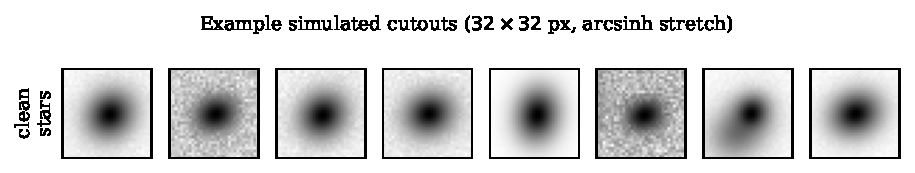
\includegraphics[width=\textwidth]{figures/fig_simdata.pdf}
\caption{Example simulated clean-star cutouts ($32\times32$ px, arcsinh stretch): the
compact point sources that inform the PSF. Galaxy detections also populate the simulated
fields but, under the point-source-context policy (\S\ref{sec:method},~\S\ref{sec:sim}),
are excluded from the attention context.\label{fig:simdata}}
\end{figure*}


\begin{figure}
\centering
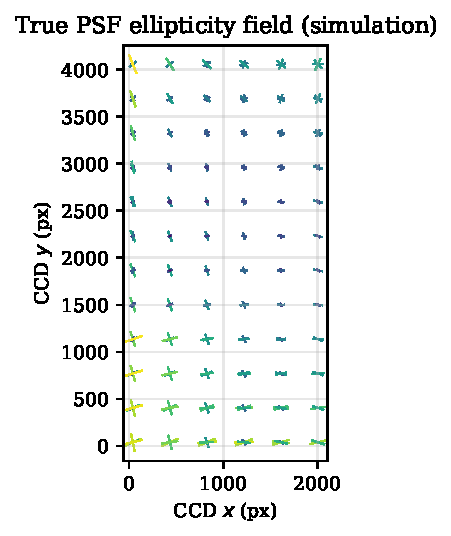
\includegraphics[width=\columnwidth]{figures/fig_psffield.pdf}
\caption{The true, spatially varying PSF ellipticity field in a simulated exposure (whisker length $\propto|e|$); the network must recover this at star-free positions.\label{fig:psffield}}
\end{figure}

\section{Results} \label{sec:results}

\subsection{Reserved-star accuracy on real data} \label{sec:headline}

On 3{,}301 test exposures and 73{,}609 reserved stars, our model (no
per-exposure fitting) matches or exceeds both baselines on every metric
(Table~\ref{tab:headline}). Every method is scored on the identical set of reserved stars.
\begin{figure*}
\centering
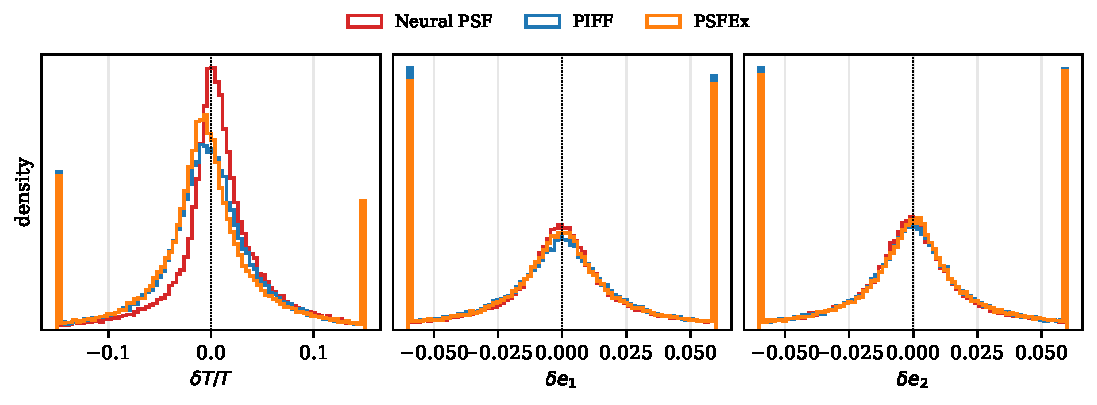
\includegraphics[width=\textwidth]{figures/fig_residuals.pdf}
\caption{Reserved-star residual distributions on the DES test split. Our model (red) is the narrowest in size and ellipticity.\label{fig:residuals}}
\end{figure*}



\begin{deluxetable}{lcccccc}
\tablecaption{Reserved-star residuals on the DES test split (3{,}301 exposures,
73{,}609 stars). $T$ scatter is the robust standard deviation of $\delta T/T$;
$|\delta e|$ are median absolute ellipticity residuals; corr is the model--star shape
correlation. Best in bold.\label{tab:headline}}
\tablehead{\colhead{Method} & \colhead{$T$ scat} & \colhead{$|\delta e_1|$} &
\colhead{$|\delta e_2|$} & \colhead{corr$(e_1)$} & \colhead{corr$(e_2)$} &
\colhead{$\chi^2/$dof}}
\startdata
\textbf{Neural PSF (ours)} & \textbf{0.0301} & \textbf{0.0151} & \textbf{0.0150} &
  \textbf{0.650} & \textbf{0.607} & 1.037 \\
\textsc{PIFF}      & 0.0393 & 0.0171 & 0.0158 & 0.611 & 0.577 & 1.073 \\
\textsc{PSFEx}     & 0.0371 & 0.0160 & 0.0154 & 0.645 & 0.604 & 1.047 \\
\enddata
\end{deluxetable}

\subsection{Pixel-level and astrometric validation} \label{sec:pixval}

Because the model regresses the effective PSF (the expected pixel values), the
reserved-star quality of fit can be assessed directly in the modeled (pixel) space,
the validation native to effective-PSF work \citep{AndersonKing2000}. Two checks
follow. First, the inverse-variance $\chi^2/$dof is a noise-calibrated goodness of
fit: at $1.04$ (Table~\ref{tab:headline}) the per-pixel residuals are consistent with
photon and read noise, i.e.\ no unmodeled pixel-level structure, a statement available
to a sub-pixel model only through its rendered output. The variance is the survey's own
inverse-weight (photon plus read noise) map, not a quantity tuned to the residuals, so
$\chi^2\!\approx\!1$ is an independent calibration check rather than a fitted outcome.
Second, the predicted ePSF
centroid matches the star centroid to $0.010$\,px ($2.6$\,mas) in median offset, versus
$0.017$\,px ($4.5$\,mas) for \textsc{PIFF} and $0.020$\,px ($5.1$\,mas) for \textsc{PSFEx}
(Table~\ref{tab:astrom}); all three centroids are measured with the same adaptive-moment
routine on the same pixel grid, so the difference reflects the models, not a centroiding
convention. This is a near $2\times$ improvement on a quantity the ePSF formalism is built
to optimize.

\begin{deluxetable}{lccc}
\tablecaption{Astrometric residual of the model PSF centroid relative to the star, on
the reserved test stars. Per-axis scatter is the robust standard deviation; the offset
is the median radius ($0.263''$/px). Best in bold.\label{tab:astrom}}
\tablehead{\colhead{Method} & \colhead{$\sigma(\delta x)$ [px]} &
\colhead{$\sigma(\delta y)$ [px]} & \colhead{median $|\delta|$ [mas]}}
\startdata
\textbf{Neural PSF (ours)} & \textbf{0.008} & \textbf{0.009} & \textbf{2.6} \\
\textsc{PIFF}      & 0.015 & 0.013 & 4.5 \\
\textsc{PSFEx}     & 0.015 & 0.017 & 5.1 \\
\enddata
\end{deluxetable}

Third, stacking the unit-normalized residual (observed star minus model, as a fraction of
total light) over $306$ reserved stars isolates any coherent shape error that second
moments can miss (Figure~\ref{fig:residstack}). Our model leaves the flattest residual
(RMS $2.6\times10^{-4}$); \textsc{PIFF} and \textsc{PSFEx} leave a visible negative core
($3.5$ and $4.4\times10^{-4}$), a higher-order mismatch in the central pixels that is
consistent with their larger size residuals and is invisible to the size and ellipticity
summaries alone.
\begin{figure*}
\centering
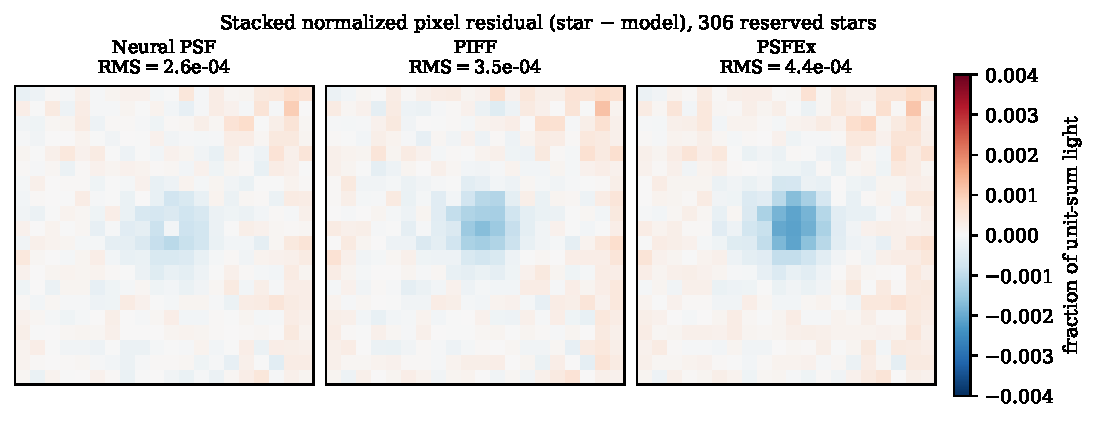
\includegraphics[width=\textwidth]{figures/fig_residual_stack.pdf}
\caption{Stacked normalized pixel residual (observed star $-$ model, unit-sum) over 306
reserved test stars, on a common scale. Our model leaves the flattest residual;
the per-exposure baselines retain a coherent central core---a higher-order shape error
that second-moment metrics do not capture (\S\ref{sec:pixval}).\label{fig:residstack}}
\end{figure*}

\subsection{Residual two-point statistics} \label{sec:rho}

Per-star residuals understate the impact on weak lensing, where the
\emph{spatially coherent} part of the PSF-modeling error sources additive shear
bias. We therefore compute the standard $\rho$-statistics
\citep{Rowe2010,Jarvis2016} of the reserved-star residuals (the auto- and
cross-correlations of the residual ellipticity $\delta e$ and the
size-leakage term $e\,\delta_T$), accumulated within exposures with
\textsc{treecorr} (Figure~\ref{fig:rho}). On the same reserved stars used for
Table~\ref{tab:headline}, our model is at or below both per-exposure
baselines on four of the five statistics: the median $|\xi_+|$ across angular
scales is $3.9\times10^{-5}$ ($\rho_1$), $5.2\times10^{-5}$ ($\rho_2$),
$2.5\times10^{-6}$ ($\rho_3$), and $4.8\times10^{-6}$ ($\rho_4$), against
$\rho_1,\rho_2\gtrsim7\times10^{-5}$ and $\rho_3\simeq6\times10^{-5}$ for
\textsc{PIFF}. The $\rho_3$ result, more than an order of magnitude below
\textsc{PIFF}, reflects the model's smaller and less spatially structured size
residuals. The one exception is $\rho_5=\langle e\,(e\,\delta_T)\rangle$, where
our model ($5.4\times10^{-5}$) sits above the baselines (${\sim}10^{-5}$): a
residual coupling between PSF shape and the size error that a weak-lensing
analysis would carry in its additive-bias budget. Overall the coherent,
lensing-relevant part of the residual is no larger than that of the per-exposure
baselines, despite our model fitting no per-exposure free parameters.
\begin{figure*}
\centering
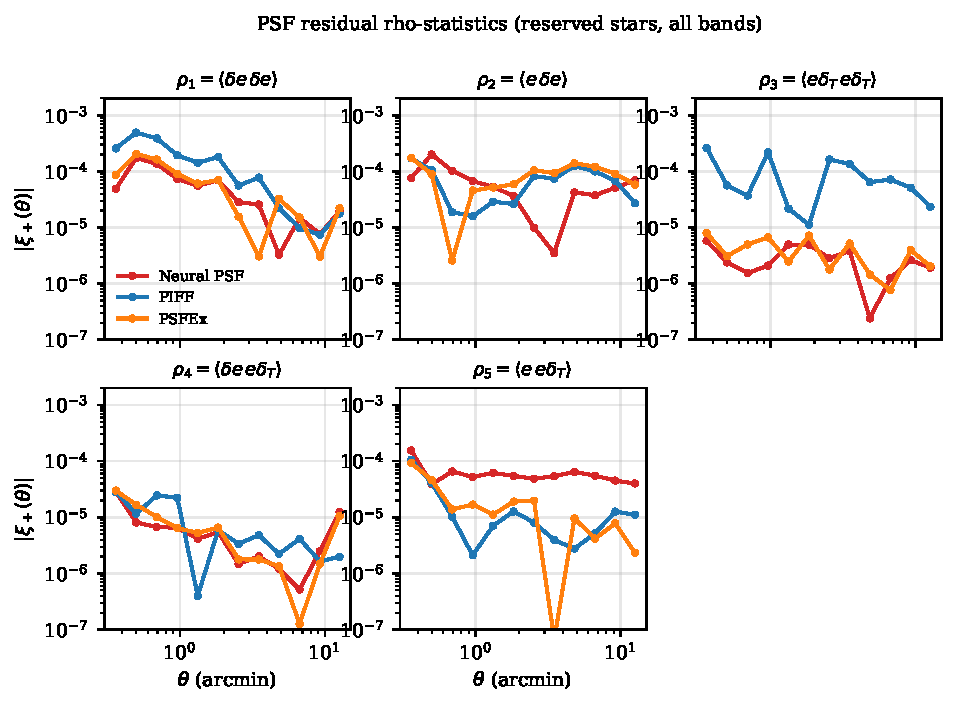
\includegraphics[width=\textwidth]{figures/fig_rho_stats.pdf}
\caption{PSF residual $\rho$-statistics on reserved stars, per method. Our model
(red) is at or below both baselines on $\rho_1$--$\rho_4$; only $\rho_5$ (the
shape--size coupling) is modestly larger (\S\ref{sec:rho}).\label{fig:rho}}
\end{figure*}

\subsection{Galaxy recovery on real data} \label{sec:galrec}

We test the inferential goal directly. We inject \textsc{galsim} galaxies, convolved with
a strictly isolated reserved star's empirical PSF, at that star's position; each method
predicts the PSF there from the \emph{other} stars and recovers the galaxy. Recovering
with the true PSF (the anchor's own image) sets the protocol floor: near-zero ellipticity
bias and a residual $-1.2\%$ size bias---not a true zero, but the discretization floor of
the recovery forward model---against which the predicted PSFs are scored.
On 32 $r$-band test exposures (170 anchors; Table~\ref{tab:galrec}), all three methods recover galaxy
\emph{ellipticity} with low bias ($|\Delta e_1|\lesssim0.013$): the pixel-convolved
effective PSF carries the PSF ellipticity faithfully into the forward model, so no method
imprints a coherent shape error on the recovered galaxies, the weak-lensing-critical
property, which our model satisfies on par with the per-exposure baselines. The methods
separate instead on recovered \emph{size}: \textsc{PIFF} is slightly large ($+1.1\%$),
while our recovered sizes are ${\sim}8\%$ small. We trace this to the \emph{flux at which
the PSF is queried}. The model conditions on source flux, and---learning from training
stars that carry faint unresolved neighbours---has encoded that fainter stars are more
fractionally contaminated; its predicted PSF therefore narrows as the query flux rises,
approaching the clean PSF in the bright limit. Queried at the median star flux, as in the
recovery above, the predicted PSF is contamination-broadened, carrying ${\sim}13\%$ too
much second-moment area (and ${\sim}2\%$ less encircled energy in the central few pixels)
relative to bright, minimally-contaminated stars; this biases recovered galaxy sizes low.
Queried instead at the clean high-flux limit, the predicted PSF size matches bright clean
reserved stars to within $1\%$---a direct HSM-size residual of $+13.4\%$ at the median flux
falling to $+0.0\pm0.4\%$ at $10^6$ (Table~\ref{tab:fluxsize})---and the recovered
galaxy-size bias collapses correspondingly: on $16$ matched held-out exposures the
de-confounded bias (implicit minus the true-PSF recovery) falls from $-5.1\%$ at the median
flux to $-0.7\%$ at the clean flux, i.e.\ essentially to the protocol floor. The clean
window is broad: the size residual is flat
from $5\times10^5$ to $6\times10^6$, brighter-fatter contributing only $+0.2\%$ across that
decade. Controlled simulations confirm the mechanism against \emph{known} truth, with no
brighter-fatter to confound: the same flux query drives the learned PSF concentration from
$\delta\mathrm{EE}=-0.0078$ at the median flux to $-0.0014$ at the clean limit
(\S\ref{sec:sim}), i.e.\ essentially onto the true PSF. That the model recovers the clean
PSF purely through its learned flux dependence is independent confirmation that
faint-neighbour contamination of the training stars is the cause. The size bias is thus
largely a query-flux effect rather than an irreducible limitation; recovered ellipticity,
the consequential quantity for shear, is unbiased throughout.
\begin{figure*}
\centering
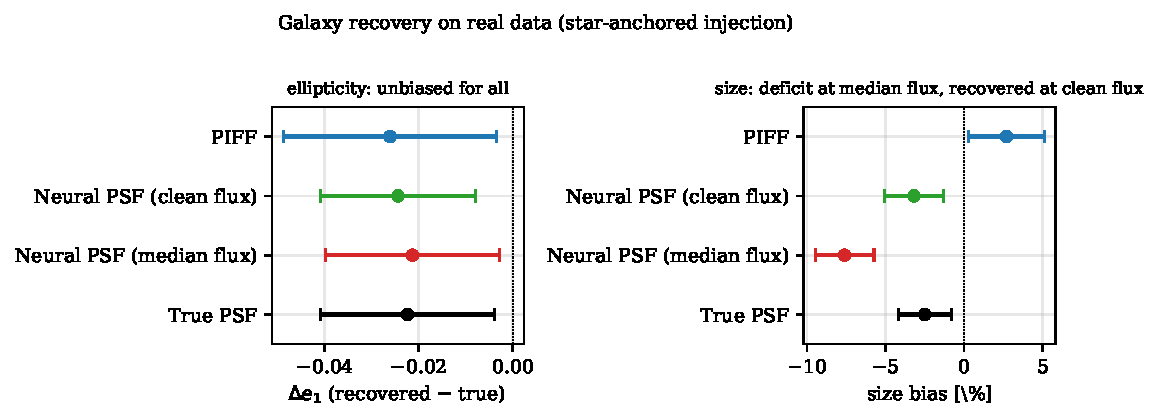
\includegraphics[width=0.75\textwidth]{figures/fig_galrec.pdf}
\caption{Galaxy recovery on real data (star-anchored injection), median $\pm$ bootstrap 95\%
CI per PSF. Left: recovered ellipticity is low-bias ($|\Delta e_1|\lesssim0.013$) for all
three methods. Right: rendered at the median query flux the methods separate on recovered
\emph{size}---our model runs ${\sim}8\%$ small (contamination-broadening of the predicted
PSF, removed by querying at the clean high-flux limit; \S\ref{sec:galrec}), while
\textsc{PIFF} and the true PSF are near zero.\label{fig:galrec}}
\end{figure*}



\begin{deluxetable}{lccc}
\tablecaption{Star-anchored galaxy injection--recovery (32 $r$-band test exposures, 170 anchors). The
true-PSF recovery sets the protocol floor. All methods recover ellipticity with low bias;
they separate on recovered size. Our model is rendered here at the median query flux; the
size deficit is largely a query-flux effect and is removed at the clean flux
(Table~\ref{tab:fluxsize}, \S\ref{sec:galrec}).\label{tab:galrec}}
\tablehead{\colhead{PSF} & \colhead{Size bias} & \colhead{$\Delta e_1$} &
\colhead{$\Delta e_2$}}
\startdata
True PSF            & $-1.2\%$ & $-0.009$ & $-0.000$ \\
\textbf{Neural PSF (ours)}  & $-7.6\%$ & $-0.005$ & $-0.000$ \\
\textsc{PIFF}       & $+1.1\%$ & $-0.013$ & $-0.003$ \\
\enddata
\end{deluxetable}

\begin{deluxetable}{lc}
\tablecaption{Predicted PSF second-moment size residual $\delta T/T$ (HSM adaptive moments)
against bright clean reserved stars, as a function of the flux at which the PSF is queried
(50 held-out $r$-band exposures, $n=260$ stars, ${\rm S/N}\ge200$; mean\,$\pm$\,s.e.m.). The
under-concentration is a query-flux effect: at the median star flux the predicted PSF is
contamination-broadened; at the clean high-flux limit it matches bright clean stars, and the
window is broad and flat ($\delta T/T$ stays within $1\%$ from $5\times10^5$ to $6\times10^6$,
brighter-fatter contributing $+0.2\%$ across that decade).\label{tab:fluxsize}}
\tablehead{\colhead{Query flux (ADU)} & \colhead{$\delta T/T$}}
\startdata
median star flux & $+13.4 \pm 0.6\%$ \\
$10^5$           & $+6.7 \pm 0.5\%$ \\
$5\times10^5$    & $+0.2 \pm 0.4\%$ \\
$10^6$           & $+0.0 \pm 0.4\%$ \\
\enddata
\end{deluxetable}

\subsection{Chromatic PSF correction} \label{sec:chromatic}

In a chromatic simulation (FWHM varies $-3\%$/mag of $g{-}i$), color conditioning reduces
the residual chromatic size slope from $-0.06$/mag (\textsc{PIFF}, \textsc{PSFEx}, and our
own zero-color ablation) to $+0.004$/mag, a ${\sim}15\times$ reduction. On real $r$-band
data the paired color-versus-zero-color slope difference is $+0.0024$/mag
(CI $[+0.0016,+0.0030]$); the baselines retain the chromatic slope because a per-exposure
empirical PSF has no access to per-star color.

\subsection{Sample efficiency} \label{sec:sampeff}

Restricting every method to $k$ randomly chosen fit stars, our model is
approximately flat in $k$ (size scatter $0.078\to0.056$, $\chi^2\sim1.1$ from $k=5$ to
$k=100$), while \textsc{PIFF} collapses below $k\approx25$ ($\chi^2=5.1$, scatter $0.18$
at $k=5$). Amortization transfers information from the training set to sparsely-populated
exposures.


\begin{figure}
\centering
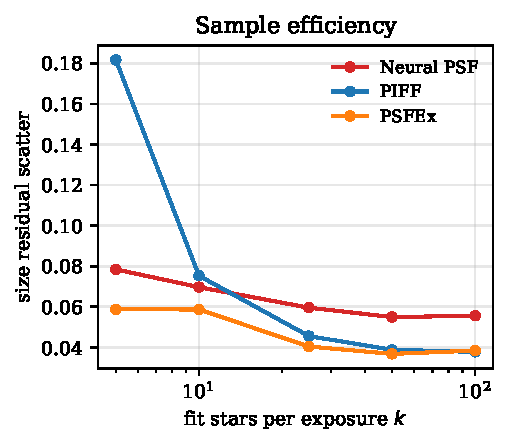
\includegraphics[width=\columnwidth]{figures/fig_sampeff.pdf}
\caption{Size-residual scatter versus the number of fit stars $k$. Our model is nearly flat in $k$; PIFF degrades sharply below $k\approx25$.\label{fig:sampeff}}
\end{figure}

\subsection{Simulation studies} \label{sec:sim}

\paragraph{Architecture ladder} On the star-free truth grid, $\chi^2/$dof improves along
additive $\to$ FiLM $\to$ diagonal $\to$ polar ($8.9\to4.96\to4.41$; \textsc{PIFF} $2.67$;
verified floor $1.0$), recovering both ellipticity components.

\paragraph{Blend forward-model} On a blended simulation, single-star training leaves a
$+4.8\%$ size bias on the star-free truth grid; the blend forward-model loss reduces it to
$+0.7\%$ (${\approx}7\times$).

\paragraph{The size deficit reproduces in simulation and is a query-flux effect} Adding the
faint-neighbour contamination of \S\ref{sec:galrec} to the training stars reproduces the
size deficit in simulation, where the truth PSF is known exactly: the learned PSF is
under-concentrated by $\delta\mathrm{EE}(r{\le}2\,{\rm px})=-0.0078$ relative to truth at
the median query flux, and injected galaxies are recovered $-2.4\%$ small (the simulation
analogue of the real deficit, after differencing against recovery through the known clean
PSF to cancel the protocol floor). Because the simulation has no brighter-fatter, the
model's only flux-dependent effect is the contamination it learned, and querying its PSF at
the clean high-flux limit---with no cleaning at all---drives $\delta\mathrm{EE}$ from
$-0.0078$ to $-0.0014$, i.e.\ essentially onto truth. This is the controlled,
truth-anchored counterpart of the real-data flux query in \S\ref{sec:galrec}, confirming
against known truth that the model's bright-limit PSF is the clean one and that the deficit
is the contamination the flux-conditioned model has implicitly learned to separate.

\paragraph{Galaxy-context corrupts PSF ellipticity---and the fix} Injecting galaxy
detections into the simulation, a model that attends to \emph{all} detections (including
galaxies) suffers a clean, reproducible failure: it cannot represent one spin-2
ellipticity component [corr$(e_1)=0.05$ under the polar parametrization; the failure flips
to $e_2$ under a Cartesian parametrization, identifying a representation degeneracy rather
than noise], while recovering the other perfectly. We localize the cause by ablation: it
is \emph{not} data volume, per-source S/N, galaxy size or color, or the $\chi^2$ cap---the
model is treating extended galaxy cutouts as PSF evidence. Restricting the attention
context to point sources recovers \emph{both} components completely
[corr$(e_1,e_2)=0.98$, matching the galaxy-free ideal]; a coordinate-system change does
not. Galaxies are clearly distinguishable (cutout second moment $T\approx33$ versus
$15\,{\rm px}^2$ for stars), so this is the model failing to use available information,
fixed by the principled restriction---which we adopt as the production policy---that only
point sources inform a PSF. Excluding galaxies from the context costs nothing measurable on
the real test set: reserved-star residuals are unchanged from the all-detections ablation
(size scatter $0.031$ versus $0.030$; identical median ellipticity error and shape
correlation), so the policy removes the simulation failure mode without trading away
real-world performance.
\begin{figure*}
\centering
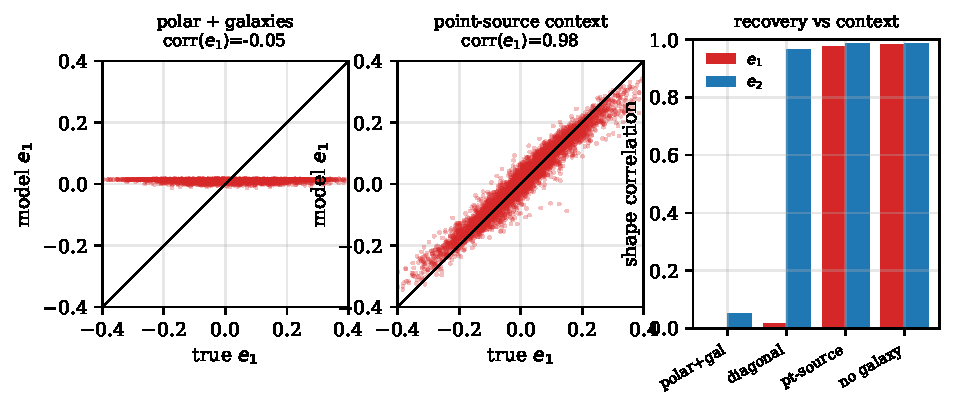
\includegraphics[width=\textwidth]{figures/fig_galaxy_context.pdf}
\caption{Galaxy detections in the attention context corrupt the recovered PSF ellipticity. Left: with galaxies in context, model $e_1$ collapses to a constant (corr$=-0.04$). Middle: restricting the context to point sources recovers it (corr$=0.98$). Right: shape correlations across configurations---point-source context and galaxy-free both recover \emph{both} components; a coordinate change (diagonal) does not.\label{fig:galcontext}}
\end{figure*}

\paragraph{Seed regularization: EMA versus ensembling} Because the field is learned once
and applied without per-exposure refitting, it carries seed-to-seed prediction noise. On the star-free truth grid we compare a single model,
an exponential moving average (EMA) of one model's weights, and a 4-seed deep ensemble
(averaging predicted stamps), each over matched 120-epoch runs (Table~\ref{tab:ema}).
EMA gives a small, consistent gain ($T$-scatter $-5\%$, ellipticity $\lesssim3\%$); the
ensemble is much larger ($-12\%$ size, $-24\%$ ellipticity). EMA is therefore \emph{not}
a substitute for ensembling: it captures only a fraction of the benefit. The per-seed
aggregate scatter is itself small (the model is seed-stable), but the per-position
predictions are diverse, which only ensembling exploits. On real reserved stars the
ensemble improves the metrics by only ${\sim}1\%$: that residual is measurement-noise- and
blend-limited (corr${\sim}0.66$, not the truth-grid $0.99$), so it masks the model-error
reduction that ensembling delivers at the star-free positions where galaxies are measured.

\begin{deluxetable}{lccc}
\tablecaption{Truth-grid PSF recovery (4 matched 120-epoch seeds): seed-noise scatter for
a single model, EMA, and a 4-seed ensemble.\label{tab:ema}}
\tablehead{\colhead{} & \colhead{$\sigma(\delta e_1)$} & \colhead{$\sigma(\delta e_2)$} &
\colhead{$\sigma(\delta T/T)$}}
\startdata
single model     & 0.0094 & 0.0099 & 0.0175 \\
EMA ($1\times$)  & 0.0092 & 0.0096 & 0.0167 \\
ensemble ($4\times$) & \textbf{0.0073} & \textbf{0.0075} & \textbf{0.0154} \\
\enddata
\end{deluxetable}

\section{Discussion} \label{sec:discussion}

Our amortized approach trades a per-exposure fit for a single trained model. Benefits: no
test-time fitting, robustness in star-sparse exposures, conditioning on color
(chromatic PSF) and flux (brighter--fatter), and a directly forward-modelable output: we
predict the pixel-convolved effective PSF, the identifiable quantity the data constrain
and the exact kernel a galaxy model is convolved with (\S\ref{sec:intro}), so the PSF
feeds a shear pipeline with no intervening pixel-deconvolution assumption. Caveats: (i)~unlike per-exposure fitters, our
approach requires many exposures to learn the field (in simulation, ellipticity
recovery is unstable below a few thousand exposures; real DES is well above this);
(ii)~the simulation's idealized PSF (Moffat, low-order polynomial field) favors the
per-exposure baselines, so absolute-accuracy comparisons rest on real data; and
(iii)~the galaxy-context finding argues that a PSF estimator's context should be gated to
point sources, which we adopt. (iv)~The model's predicted PSF \emph{size depends on the
flux at which it is queried}: it conditions on flux and has learned, from training stars
that carry faint unresolved neighbours, that fainter stars are more fractionally
contaminated and hence broader, so its predicted PSF narrows toward the clean PSF as the
query flux rises. Queried at the median star flux---which a naive galaxy-recovery render
uses---the predicted PSF is contamination-broadened (a second-moment size ${\sim}13\%$
large, ${\sim}2\%$ low in central encircled energy, relative to bright clean stars) and
biases recovered galaxy sizes a few percent low; queried at the clean high-flux limit it
matches bright clean stars to $1\%$, the size residual falling from $+13\%$ to $0\%$ across
the flux range, and the galaxy-size bias largely vanishes (\S\ref{sec:galrec}). The
flux--size trend is visible directly in the reserved-star metric (Fig.~\ref{fig:residmag}),
$\delta T/T$ rising at faint magnitudes. Controlled simulations with known truth confirm the
mechanism and that the clean-flux PSF is the true one ($\delta\mathrm{EE}$ from $-0.0078$ to
$-0.0014$; \S\ref{sec:sim}), and the effect is absent at any decoder capacity in clean
simulations, ruling out a generic spectral-bias limitation of the decoder. We identify
faint-neighbour contamination of the nominally-clean training stars as the cause, and the
practical prescription---render the inferential PSF at the clean-flux limit---removes most
of it, the main residual systematic to control before a shear analysis. As a principled
cross-check we also fit the contamination explicitly, by a Monte Carlo expectation
maximization \citep{dempster1977em,wei1990mcem} that infers each star's contaminant
posterior (with the contamination rate inferred jointly across stars rather than assumed)
and retrains the field against the cleaned stars; in controlled simulations this reaches the
same truth as the flux query, to within the seed scatter, confirming the mechanism but not
improving on the simpler query, which we therefore adopt as the operative correction.

\section{Conclusion} \label{sec:conclusion}

A single attention-based continuous PSF field, trained across DES single-epoch exposures
and applied with no per-exposure fitting, matches or exceeds \textsc{PIFF} and
\textsc{PSFEx} on real reserved stars and recovers galaxy ellipticity without coherent
bias (on par with \textsc{PIFF}) on a star-anchored injection test, while additionally
correcting a chromatic systematic and remaining robust in star-sparse exposures. The one
residual---recovered galaxy sizes a few percent small---we trace to the flux at which the
PSF is queried: the flux-conditioned model has learned that fainter stars are more
contaminated, so rendering the PSF at the clean high-flux limit removes most of the bias.
Controlled simulations motivate two further training choices: a blend forward-model loss and
point-source-only attention context. The latter follows from diagnosing a spin-2
representation failure triggered by galaxy detections in context.

\begin{acknowledgments}
This material is based on work supported by the National Science Foundation under Grant
No.~2209720 and the U.S.\ Department of Energy, Office of Science, Office of High Energy
Physics under Award Number DE-SC0023714.

This paper has undergone internal review in the LSST Dark Energy Science Collaboration.
% The internal reviewers were \ldots.                        % optional but recommended
% Author contribution statements (standard papers only).
% A.B.C.\ acknowledges support from grant \ldots\ (standard papers only).

The DESC acknowledges ongoing support from the Institut National de
Physique Nucl\'eaire et de Physique des Particules in France; the
Science \& Technology Facilities Council in the United Kingdom; and the
Department of Energy and the LSST Discovery Alliance
in the United States.  DESC uses resources of the IN2P3
Computing Center (CC-IN2P3--Lyon/Villeurbanne - France) funded by the
Centre National de la Recherche Scientifique; the National Energy
Research Scientific Computing Center, a DOE Office of Science User
Facility supported by the Office of Science of the U.S.\ Department of
Energy under Contract No.\ DE-AC02-05CH11231; STFC DiRAC HPC Facilities,
funded by UK BEIS National E-infrastructure capital grants; and the UK
particle physics grid, supported by the GridPP Collaboration.  This
work was performed in part under DOE Contract DE-AC02-76SF00515.

This project used public archival data from the Dark Energy Survey (DES). Funding for the DES Projects has been provided by the U.S. Department of Energy, the U.S. National Science Foundation, the Ministry of Science and Education of Spain, the Science and Technology FacilitiesCouncil of the United Kingdom, the Higher Education Funding Council for England, the National Center for Supercomputing Applications at the University of Illinois at Urbana-Champaign, the Kavli Institute of Cosmological Physics at the University of Chicago, the Center for Cosmology and Astro-Particle Physics at the Ohio State University, the Mitchell Institute for Fundamental Physics and Astronomy at Texas A\&M University, Financiadora de Estudos e Projetos, Funda{\c c}{\~a}o Carlos Chagas Filho de Amparo {\`a} Pesquisa do Estado do Rio de Janeiro, Conselho Nacional de Desenvolvimento Cient{\'i}fico e Tecnol{\'o}gico and the Minist{\'e}rio da Ci{\^e}ncia, Tecnologia e Inova{\c c}{\~a}o, the Deutsche Forschungsgemeinschaft, and the Collaborating Institutions in the Dark Energy Survey.

The Collaborating Institutions are Argonne National Laboratory, the University of California at Santa Cruz, the University of Cambridge, Centro de Investigaciones Energ{\'e}ticas, Medioambientales y Tecnol{\'o}gicas-Madrid, the University of Chicago, University College London, the DES-Brazil Consortium, the University of Edinburgh, the Eidgen{\"o}ssische Technische Hochschule (ETH) Z{\"u}rich,  Fermi National Accelerator Laboratory, the University of Illinois at Urbana-Champaign, the Institut de Ci{\`e}ncies de l'Espai (IEEC/CSIC), the Institut de F{\'i}sica d'Altes Energies, Lawrence Berkeley National Laboratory, the Ludwig-Maximilians Universit{\"a}t M{\"u}nchen and the associated Excellence Cluster Universe, the University of Michigan, the National Optical Astronomy Observatory, the University of Nottingham, The Ohio State University, the OzDES Membership Consortium, the University of Pennsylvania, the University of Portsmouth, SLAC National Accelerator Laboratory, Stanford University, the University of Sussex, and Texas A\&M University.

Based in part on observations at Cerro Tololo Inter-American Observatory, National Optical Astronomy Observatory, which is operated by the Association of Universities for Research in Astronomy (AURA) under a cooperative agreement with the National Science Foundation.


Baselines: \textsc{PIFF} (PixelGrid,
second-order \texttt{BasisPolynomial}, $4\sigma$ rejection) and \textsc{PSFEx}
(\texttt{PSF\_SAMPLING}~0.5, $45\times45$, \texttt{PSFVAR\_DEGREES}~2; rendered via
\textsc{galsim} \texttt{DES\_PSFEx}, \texttt{method='no\_pixel'}).
\end{acknowledgments}

\software{Astropy \citep{Astropy2022}, GalSim \citep{Rowe2015}, SEP \citep{Barbary2016},
PyTorch \citep{Paszke2019}, PIFF \citep{Jarvis2021}, PSFEx \citep{Bertin2011}}


\appendix

\section{Real-data star selection and PSF examples}\label{app:examples}

Figure~\ref{fig:selection} shows a region of a real DES single-epoch $r$-band exposure
with the source selection overlaid: clean stars used for fitting and scoring (green),
held-out reserved stars (blue), and additional context-only stellar detections (orange).
Galaxies (the extended sources, e.g.\ the bright object near the center) are detected but
excluded from the attention context (\S\ref{sec:method}).
Figure~\ref{fig:psfcompare} compares, for a single high-S/N reserved test star, the
observed stamp against the PSFEx, PIFF, and Neural PSF models evaluated at that position
(each method having seen only the non-reserved stars). All three reproduce the stellar
profile; PIFF's per-exposure interpolation is visibly noisier in the wings.

\begin{figure}
\centering
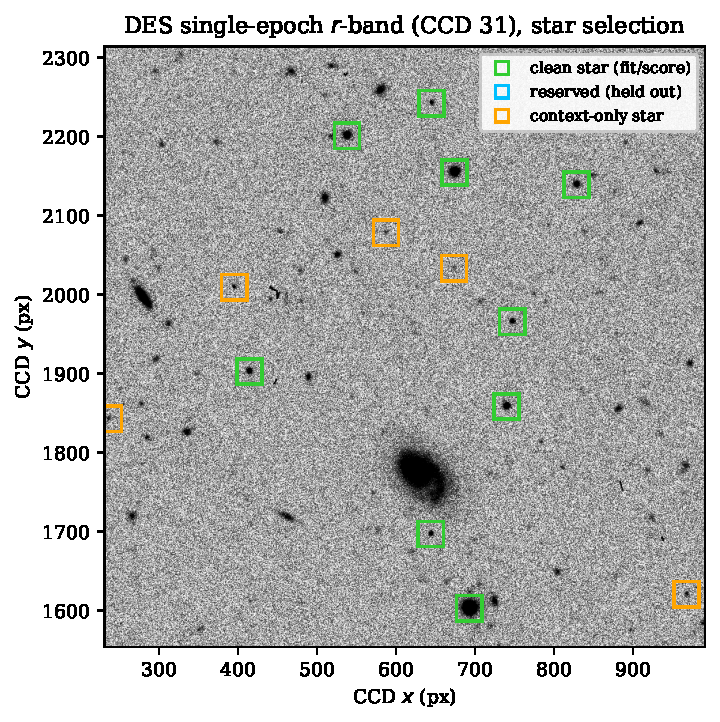
\includegraphics[width=\columnwidth]{figures/fig_des_selection.pdf}
\caption{Star selection on a real DES exposure. Green: clean stars (fit and score).
Blue: reserved (held out for evaluation). Orange: context-only stellar detections.
Extended sources (galaxies) are excluded from the attention context.\label{fig:selection}}
\end{figure}

\begin{figure*}
\centering
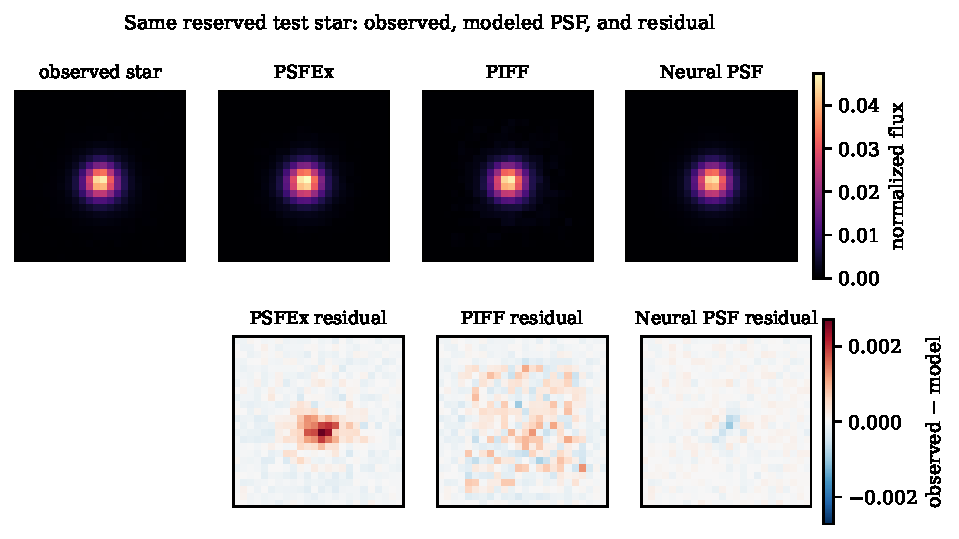
\includegraphics[width=\textwidth]{figures/fig_psf_comparison.pdf}
\caption{Top: the same reserved test star (left, observed) and the PSF predicted at its
position by PSFEx, PIFF, and Neural PSF, on a common linear stretch. Bottom: the residual
(observed $-$ model) for each method, on a common diverging scale. Each model was
fit/conditioned on the non-reserved stars only.\label{fig:psfcompare}}
\end{figure*}


\section{Benchmark validation diagnostics}\label{app:benchmark}

For comparison with standard per-exposure PSF validation \citep[cf.][]{Jarvis2021}, we report the same diagnostics.

Table~\ref{tab:perband} breaks the metrics down by band. Our
model has the smallest size scatter and median ellipticity error in every band.

\begin{deluxetable}{llccc}
\tablecaption{Reserved-star residuals by band (test split). $T$ scatter is the
robust standard deviation of $\delta T/T$; $|\delta e_1|$ is the median absolute
$e_1$ residual; corr is the model--star $e_1$ correlation. Best per band in
bold.\label{tab:perband}}
\tablehead{\colhead{Band} & \colhead{Method} & \colhead{$T$ scat} &
\colhead{$|\delta e_1|$} & \colhead{corr$(e_1)$}}
\startdata
$g$ & \textbf{Neural PSF (ours)} & \textbf{0.0331} & \textbf{0.0164} & \textbf{0.475} \\
    & \textsc{PIFF}  & 0.0439 & 0.0188 & 0.448 \\
    & \textsc{PSFEx} & 0.0417 & 0.0173 & 0.473 \\
\hline
$r$ & \textbf{Neural PSF (ours)} & \textbf{0.0291} & \textbf{0.0144} & \textbf{0.576} \\
    & \textsc{PIFF}  & 0.0366 & 0.0164 & 0.535 \\
    & \textsc{PSFEx} & 0.0340 & 0.0151 & 0.572 \\
\hline
$i$ & \textbf{Neural PSF (ours)} & \textbf{0.0274} & \textbf{0.0136} & \textbf{0.643} \\
    & \textsc{PIFF}  & 0.0342 & 0.0155 & 0.605 \\
    & \textsc{PSFEx} & 0.0339 & 0.0144 & 0.637 \\
\hline
$z$ & \textbf{Neural PSF (ours)} & \textbf{0.0272} & \textbf{0.0140} & \textbf{0.601} \\
    & \textsc{PIFF}  & 0.0387 & 0.0160 & 0.503 \\
    & \textsc{PSFEx} & 0.0359 & 0.0152 & 0.589 \\
\hline
$Y$ & \textbf{Neural PSF (ours)} & \textbf{0.0391} & \textbf{0.0210} & \textbf{0.568} \\
    & \textsc{PIFF}  & 0.0513 & 0.0226 & 0.523 \\
    & \textsc{PSFEx} & 0.0449 & 0.0221 & 0.550 \\
\enddata
\end{deluxetable}

\begin{figure*}
\centering
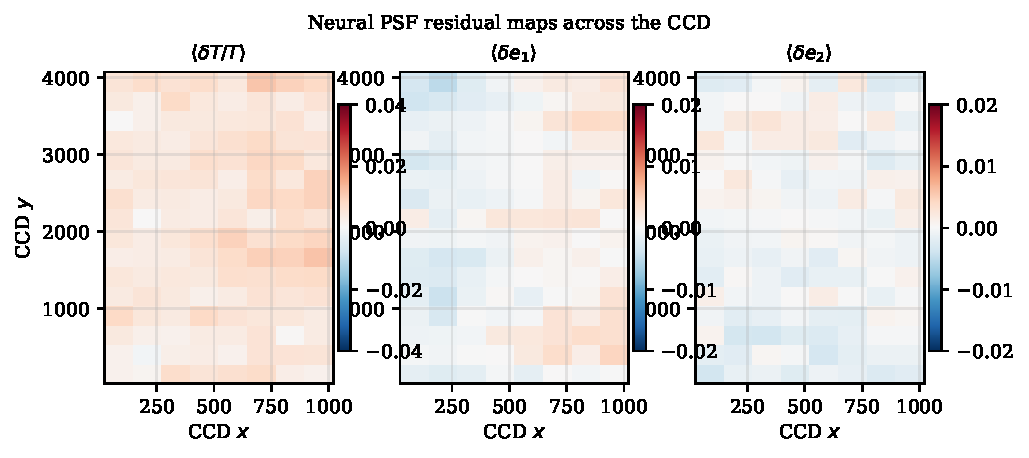
\includegraphics[width=\textwidth]{figures/fig_spatial_residuals.pdf}
\caption{Median Neural PSF residuals binned across the CCD (cf.\ PIFF Fig.~9).\label{fig:spatialres}}
\end{figure*}

\begin{figure}
\centering
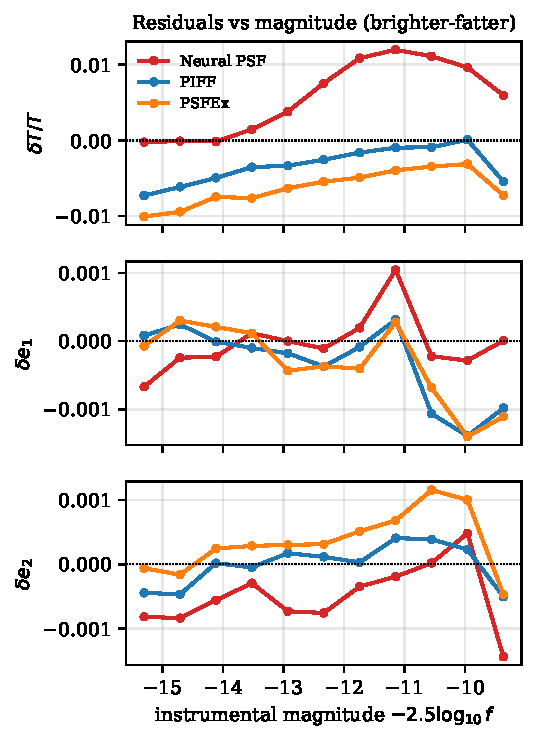
\includegraphics[width=\columnwidth]{figures/fig_resid_vs_mag.pdf}
\caption{Residuals versus instrumental magnitude (cf.\ PIFF Fig.~10). Our model (red) carries a magnitude-dependent size residual peaking at ${+}1.2\%$ (\S\ref{sec:discussion}).\label{fig:residmag}}
\end{figure}

\begin{figure}
\centering
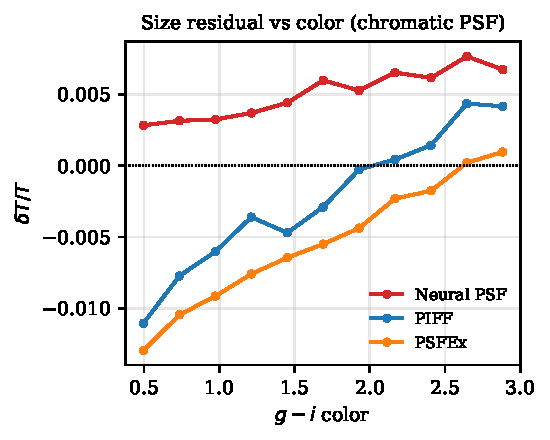
\includegraphics[width=\columnwidth]{figures/fig_resid_vs_color.pdf}
\caption{Size residual versus $g-i$ color (cf.\ PIFF Fig.~11); color conditioning keeps our chromatic residual flat.\label{fig:residcolor}}
\end{figure}

\begin{figure*}
\centering
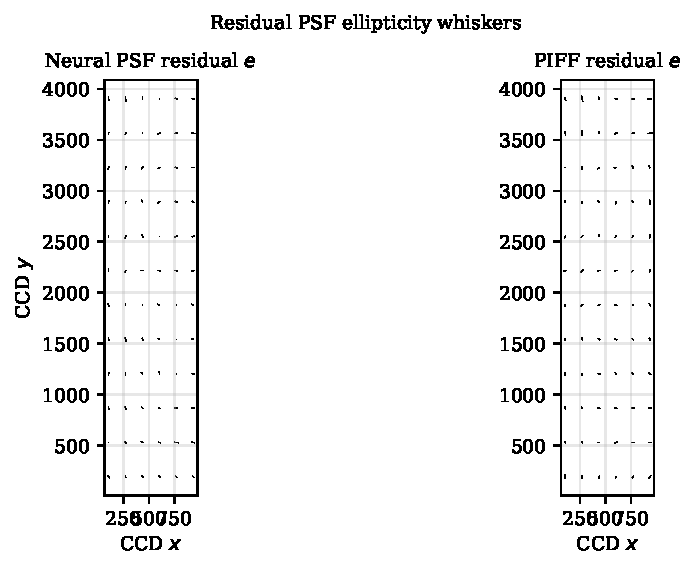
\includegraphics[width=\textwidth]{figures/fig_whisker_resid.pdf}
\caption{Residual PSF-ellipticity whiskers across the CCD, Neural PSF and PIFF (cf.\ PIFF Fig.~2).\label{fig:whisker}}
\end{figure*}

\clearpage  % flush pending appendix floats so all figures place and their labels resolve

\bibliographystyle{aasjournalv7}
\bibliography{references}

\end{document}
